\documentclass[11pt]{article}
\usepackage[utf8]{inputenc}	% Para caracteres en español
\usepackage{amsmath,amsthm,amsfonts,amssymb,amscd}
\usepackage{multirow,booktabs}
\usepackage[table]{xcolor}
\usepackage{fullpage}
\usepackage{lastpage}
\usepackage{enumitem}
\usepackage{fancyhdr}
\usepackage{mathrsfs}
\usepackage{wrapfig}
\usepackage{setspace}
\usepackage{calc}
\usepackage{multicol}
\usepackage{cancel}
\usepackage{float}
\usepackage{physics}
\usepackage[retainorgcmds]{IEEEtrantools}
\usepackage[margin=1cm]{geometry}
\usepackage{amsmath}
\newlength{\tabcont}
\setlength{\parindent}{0.0in}
\setlength{\parskip}{0.05in}
\usepackage{empheq}
\usepackage{framed}
\usepackage[most]{tcolorbox}
\usepackage{xcolor}
\usepackage[version=3]{mhchem}
\usepackage[english]{babel}
\usepackage[utf8]{inputenc}
\usepackage{graphicx}
\usepackage[colorinlistoftodos]{todonotes}

\colorlet{shadecolor}{orange!15}
\parindent 0in
\parskip 12pt
\geometry{margin=1in, headsep=0.25in}
\theoremstyle{definition}
\newtheorem{defn}{Definition}
\newtheorem{reg}{Rule}
\newtheorem{exer}{Exercise}
\newtheorem{note}{Note}
\begin{document}
\setcounter{section}{2}
%\setcounter{subsection}{}
\title{Problem Set 1}

%==============================================================
%\thispagestyle{empty}

\begin{center}
{\LARGE \bf Problem Set 1}\\
{\large Physics 180}\\
Martin 3rd Ed
\end{center}

\begin{figure}[h!]
    \centering
    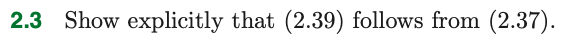
\includegraphics[scale = 0.5]{2.3.png}
\end{figure}

Equation 2.37 gives an expression for the form factor:

\begin{equation*}
    F(\mathbf{q}^2) = \frac{1}{Ze}\int f(\mathbf{r})\sum_{n=0}^{\infty} \frac{1}{n!} \left(\frac{i|\mathbf{q}|r\cos\theta}{\hbar}\right)^n \; d^3\mathbf{r} \tag{2.37}
\end{equation*}

from here on, we can assume spherical symmetry to expand $d^3\mathbf{r} = r^2 \sin\theta dr d\theta d\phi$ where it appears, and have $f(\mathbf{r}) \rightarrow f(r)$:

\begin{equation*}
    F(\mathbf{q}^2) = \frac{1}{Ze}\int_{\theta=0}^{\theta=\pi}\int_{r=0}^{r=\infty} f(r)\sum_{n=0}^{\infty} \frac{1}{n!} \left(\frac{i|\mathbf{q}|r\cos\theta}{\hbar}\right)^n \; r^2 \sin\theta dr d\theta  \int_{\phi=0}^{\phi=2\pi} d\phi \tag{2.37.1}
\end{equation*}

\begin{equation*}
    F(\mathbf{q}^2) = \frac{2\pi}{Ze}\int_{\theta=0}^{\theta=\pi}\int_{r=0}^{r=\infty} f(r)\sum_{n=0}^{\infty} \frac{1}{n!} \left(\frac{i|\mathbf{q}|r\cos\theta}{\hbar}\right)^n \; r^2 \sin\theta dr d\theta\tag{2.37.2}
\end{equation*}

we expand to show the first few terms of the summation:

\begin{align*}
    F(\mathbf{q}^2) = \frac{2\pi}{Ze}\int_{\theta=0}^{\theta=\pi}\int_{r=0}^{r=\infty} f(r)
    \biggl[r^2 \sin\theta dr d\theta&+
        \frac{i|\mathbf{q}|}{\hbar}r^3\cos\theta\; dr \; \sin\theta \; d\theta
        \\
        &-
        \frac{|\mathbf{q}|^2}{2\hbar^2} r^4\; dr  \cos^2\theta\sin\theta \;  d\theta
        + \dots \biggr]  \tag{2.37.3}
\end{align*}

\begin{align*}
    F(\mathbf{q}^2) = \frac{2\pi}{Ze}\int_{r=0}^{r=\infty} f(r)
    \biggl[2r^2 dr &-
        \frac{|\mathbf{q}|^2}{3\hbar^2} r^4\; dr 
    + \dots  \biggr]\tag{2.37.4}
\end{align*}

\begin{align*}
    F(\mathbf{q}^2) = 
    \frac{4\pi}{Ze}\int_{r=0}^{r=\infty} f(r) r^2 dr
    - 
    \frac{2\pi|\mathbf{q}|^2}{3Ze\hbar^2}\int_{r=0}^{r=\infty} f(r)r^4\; dr + \dots
    \tag{2.37.5}\label{2.37.5}
\end{align*}

from Equation 2.23 we have an expression for $Ze$ as a static charge distribution (a.k.a. the normalization condition):

\begin{align*}
    \int f(\mathbf{r}) d^3 \mathbf{r} = Ze \tag{2.23}
\end{align*}

expanding in spherical coordinates once more, we have:

\begin{align*}
    \int_{r=0}^{r=\infty} f(r) r^2 \; dr \; \int_{\theta=0}^{\theta=\pi} \sin\theta d\theta\;  \int_{\phi=0}^{\phi=2\pi} d\phi = Ze \tag{2.23.1}
\end{align*}

\begin{align*}
    4\pi \int_{r=0}^{r=\infty} f(r) r^2  \; dr  = Ze \tag{2.23.1}
\end{align*}

the left hand side is the same as the first term of Equation \ref{2.37.5}, thus we get:

\begin{align*}
    F(\mathbf{q}^2) = 
    \cancelto{1}{4\pi\int_{r=0}^{r=\infty} f(r) r^2 dr \left( 4\pi \int_{r=0}^{r=\infty} f(r) r^2 \; dr \right)^{-1}}
    - 
    \frac{2\pi|\mathbf{q}|^2}{3Ze\hbar^2}\int_{r=0}^{r=\infty} f(r)r^4\; dr + \dots
    \tag{2.37.6}\label{2.37.6}
\end{align*}

\begin{align*}
    F(\mathbf{q}^2) = 
    1
    - 
    \frac{2\pi|\mathbf{q}|^2}{3Ze\hbar^2}\int_{r=0}^{r=\infty} f(r)r^4\; dr + \dots
    \tag{2.37.7}\label{2.37.7}
\end{align*}

from Equation 2.36 we have an expression for mean square charge radius:

\begin{align*}
    \expval{r^2} = \frac{1}{Ze} \int r^2 f(\mathbf{r}) d^3 \mathbf{r} \tag{2.36}
\end{align*}

expanding again in spherical coordinates, this becomes:

\begin{align*}
    \expval{r^2} = \frac{1}{Ze} \int_{r=0}^{r=\infty} r^4 f(r) \; dr \; \int_{\theta=0}^{\theta=\pi} \sin\theta d\theta\;  \int_{\phi=0}^{\phi=2\pi} d\phi\tag{2.36.1}
\end{align*}

\begin{align*}
    \expval{r^2} = \frac{4\pi}{Ze} \int_{r=0}^{r=\infty} r^4 f(r) \; dr \tag{2.36.2}
\end{align*}

we can insert this into the second term of Equation \ref{2.37.7} and get:

\begin{align*}
    F(\mathbf{q}^2) = 
    1
    - 
    \left(\frac{4\pi}{Ze}\int_{r=0}^{r=\infty} f(r)r^4 \; dr \right)\frac{|\mathbf{q}|^2}{6\hbar^2} + \dots
    \tag{2.38.1}\label{2.38.1}
\end{align*}

\begin{align*}
    F(\mathbf{q}^2) = 
    1
    - 
    \frac{|\mathbf{q}|^2}{6\hbar^2}\expval{r^2} + \dots
    \tag{2.38.2}
\end{align*}

we can drop the absolute value sign and thus arrive at Equation 2.39:

\begin{equation*}
    \boxed{
        F(\mathbf{q}^2) = 1 - \frac{\mathbf{q}^2}{6\hbar^2}\expval{r} + \dots \tag{2.39}
    }
\end{equation*}
\newpage
%==============================================================
\setcounter{equation}{1}
\begin{figure}[h!]
    \centering
    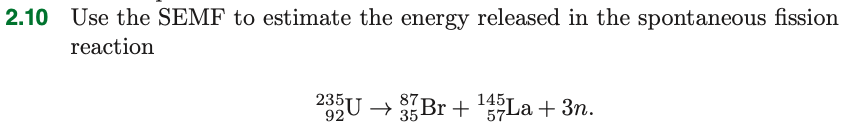
\includegraphics[scale = 0.45]{2.10.png}
\end{figure}

To obtain the released energy, we get difference between the binding energies B of the products and the reactant:
\begin{align*}
    E &= (\text{B}_{\text{Br}} + \text{B}_{\text{La}}) - \text{B}_{\text{U}} \tag{2.48.1}\\
    E &= [ \text{B}(35,87) + \text{B}(57,145) ] - \text{B}(92,235) \tag{2.48.2}
\end{align*}

we proceed to approximate each binding energy B by getting their respective atomic masses with SEMF as given by Equation 2.49:

\begin{equation*}
    \text{M}(\text{Z},\text{A}) = \sum_{i=0}^{5} f_i(\text{Z},\text{A}) \tag{2.49}
\end{equation*}

where each $f_i(\text{Z},\text{A})$ is:

\begin{align*}
    f_0(\text{Z},\text{A}) &= \text{Z}(M_p + m_e) + (\text{A}-\text{Z})M_n \tag{2.50}\\
    f_1(\text{Z},\text{A}) &= -a_v  A \tag{2.51}\\
    f_2(\text{Z},\text{A}) &= a_s A^{2/3} \tag{2.52}\\
    %f_3(\text{Z},\text{A}) &= a_c \frac{Z(Z-1)}{A^{1/3}} \tag{2.53}\\
    f_3(\text{Z},\text{A}) &= a_c \frac{Z^2}{A^{1/3}} \tag{2.53}\\
    f_4(\text{Z},\text{A}) &= a_a \frac{(Z-A/2)^2}{A} \tag{2.54}\\
    f_5(\text{Z},\text{A}) &= -f(A)\;\;\; \text{if both } Z,N \text{ are even} \\
    &= +f(A)\;\;\; \text{if both } Z,N \text{ are odd} \tag{2.55}\\
    &= 0 \;\;\; \text{ if either one of } Z,N \text{ is odd and the other is even } \\
\end{align*}

where $N=A-Z$ and $f(A) = a_p A^{-1/2}$ is usually used for Equation 2.55. Getting each atomic mass we have:

\begin{align*}
    &\text{M}(92,235) \\
    &=  92(M_p + m_e) + 143M_n - 235a_v + 235^{2/3}a_s + \frac{92^2}{235^{1/3}}a_c + \frac{(92-\frac{235}{2})^2}{235}a_a + 0 \tag{2.56.1}
\end{align*}

\begin{align*}
    &\text{M}(35,87) \\
    &=  35(M_p + m_e) + 52M_n - 87a_v + 87^{2/3}a_s + \frac{35^2}{87^{1/3}}a_c + \frac{(35-\frac{87}{2})^2}{87}a_a + 0 \tag{2.56.2}
\end{align*}

\begin{align*}
    &\text{M}(57,145)  \\
    &=  57(M_p + m_e) + 88M_n - 145a_v + 145^{2/3}a_s + \frac{57^2}{145^{1/3}}a_c + \frac{(57-\frac{145}{2})^2}{145}a_a + 0 \tag{2.56.3}
\end{align*}

%DRAFT
%\begin{align*}
%    &\text{M}(92,235) \\
%    &=  92(M_p + m_e) + 143M_n - 235a_v + 235^{2/3}a_s + \frac{(92)(91)}{235^{1/3}}a_c + \frac{(92-\frac{235}{2})^2}{235}a_a + 0 \tag{2.56.1}
%\end{align*}

%\begin{align*}
%    &\text{M}(35,87) \\
%    &=  35(M_p + m_e) + 52M_n - 87a_v + 87^{2/3}a_s + \frac{(35)(34)}{87^{1/3}}a_c + \frac{(35-\frac{87}{2})^2}{87}a_a + 0 \tag{2.56.2}
%\end{align*}

%\begin{align*}
%    &\text{M}(57,145)  \\
%    &=  57(M_p + m_e) + 88M_n - 145a_v + 145^{2/3}a_s + \frac{(57)(56)}{145^{1/3}}a_c + \frac{(57-\frac{145}{2})^2}{145}a_a + 0 \tag{2.56.3}
%\end{align*}

using these, we can get the binding energies using Equation 2.48:

\begin{align*}
    \text{B}(\text{Z},\text{A}) = -\frac{1}{c^2}[\text{M}(\text{Z},\text{A}) - \text{Z}(M_p+m_e) - \text{N}M_n] \tag{2.48}
\end{align*}

for convenience we absorb the $1/c^2$ into the $a_i$ constants, thus we have:

\begin{align*}
    &\text{B}(92,235) = 235a_v - 235^{2/3}a_s - \frac{92^2}{235^{1/3}}a_c - \frac{(92-\frac{235}{2})^2}{235}a_a - 0 \tag{2.57.1}
\end{align*}

\begin{align*}
    &\text{B}(35,87) = 87a_v - 87^{2/3}a_s - \frac{35^2}{87^{1/3}}a_c - \frac{(35-\frac{87}{2})^2}{87}a_a - 0 \tag{2.57.2}
\end{align*}

\begin{align*}
    &\text{B}(57,145) = 145a_v - 145^{2/3}a_s - \frac{57^2}{145^{1/3}}a_c - \frac{(57-\frac{145}{2})^2}{145}a_a - 0 \tag{2.57.3}
\end{align*}

%DRAFT
%\begin{align*}
%    &\text{B}(92,235) =  + 235a_v - 235^{2/3}a_s - \frac{(92)(91)}{235^{1/3}}a_c - \frac{(92-\frac{235}{2})^2}{235}a_a - 0 \tag{2.57.1}
%\end{align*}

%\begin{align*}
%    &\text{B}(35,87)   + 87a_v + 87^{2/3}a_s - \frac{(35)(34)}{87^{1/3}}a_c - \frac{(35-\frac{87}{2})^2}{87}a_a - 0 \tag{2.57.2}
%\end{align*}

%\begin{align*}
%    &\text{B}(57,145)  =  + 145a_v + 145^{2/3}a_s - \frac{(57)(56)}{145^{1/3}}a_c - \frac{(57-\frac{145}{2})^2}{145}a_a - 0 \tag{2.57.3}
%\end{align*}

getting energy released E per Equation 2.48.2:

\begin{align*}
    E &= [87+145-235]a_v\\
    &+ [-87^{2/3} - 145^{2/3} + 235^{2/3}]a_s\\
    &+ \left[ -\frac{35^2}{87^{1/3}} - \frac{57^2}{145^{1/3}} + \frac{92^2}{235^{1/3}}\right]a_c \tag{2.57.4}\\
    &+ \left[ -\frac{(35-\frac{87}{2})^2}{87} - \frac{(57-\frac{145}{2})^2}{145} + \frac{(92-\frac{235}{2})^2}{235}\right]a_a
\end{align*}

%DRAFT
%\begin{align*}
%    E &= [87+145-235]a_v\\
%    &+ [-87^{2/3} - 145^{2/3} + 235^{2/3}]a_s\\
%    &+ \left[ -\frac{(35)(34)}{87^{1/3}} - \frac{(57)(56)}{145^{1/3}} + \frac{(92)(91)}{235^{1/3}}\right]a_c\\
%    &+ \left[ -\frac{(35-\frac{87}{2})^2}{87} - \frac{(57-\frac{145}{2})^2}{145} + \frac{(92-\frac{235}{2})^2}{235}\right]a_a
%\end{align*}

\begin{align*}
    E &= -3a_v - 9.15a_s + 476.68 a_c + 0.28a_a \tag{2.57.5}
\end{align*}

%DRAFT
%\begin{align*}
%    E &= -3a_v - 9.15a_s + 480.52 a_c + 0.28a_a
%\end{align*}

we use the following values for the $a_i$ terms (in $MeV/c^2$ units):

\begin{align*}
    a_v = 15.56,\;\;\; a_s = 17.23,\;\;\; a_c = 0.697,\;\;\; a_a = 93.14 \tag{2.58}
\end{align*}

thus for released energy we have:

\begin{equation*}
\boxed{
    E = 154.00\; MeV
}
\end{equation*}

%480.5227247
\end{document}